%!TEX program = xelatex
\documentclass{beamer}

\usepackage{blindtext}

\usepackage[T1]{fontenc}
\usepackage[font=small,labelfont=bf,tableposition=top]{caption}
\renewcommand{\figurename}{}
\usepackage{graphicx}



\usetheme{Execushares}

\title{Sistema Integrado de Consulta a Licitações Públicas}
\subtitle{Alex Sandro da Silva Magalhães Junior,\\ André Lucas Rodrigues da Silva}

\author{Instituto Federal de Goiás - Câmpus Formosa 2018}
\date{}
\setcounter{showSlideNumbers}{1}

\begin{document}
	\setcounter{showProgressBar}{0}
	\setcounter{showSlideNumbers}{0}

	\frame{\titlepage}

	\begin{frame}
		\frametitle{Agenda}
		\begin{enumerate}
			\item Processo Licitatório\\ %\textcolor{ExecusharesGrey}{\footnotesize\hspace{1em} Histórico}\\
			%\textcolor{ExecusharesGrey}{\footnotesize\hspace{1em} No Brasil}\\
			%\textcolor{ExecusharesGrey}{\footnotesize\hspace{1em} Definição}\\
			%\textcolor{ExecusharesGrey}{\footnotesize\hspace{1em} Processo Licitatório Contemporâneo}
			\textcolor{ExecusharesGrey}{\footnotesize\hspace{1em} Histórico, Definição e o Processo Contemporâneo}\\
			\item Fase Interna do Processo Licitatório\\
			\textcolor{ExecusharesGrey}{\footnotesize\hspace{1em} Como funciona}\\
			\item Análise e Desenvolvimento de Sistemas \\
			\textcolor{ExecusharesGrey}{\footnotesize\hspace{1em} Metodologia, ferramentas e tecnologias}\\
			 %\textcolor{ExecusharesGrey}{\footnotesize\hspace{1em} Visão Geral}\\
			%\begin{itemize}
				%\item Metodologias de desenvolvimento de software\\ 
				%\item Levantamento de requisitos\\ 
				%\item Implementação\\ %\textcolor{ExecusharesGrey}{\footnotesize\hspace{1em} Conceitos e Tecnologias}
				%\item Homologação e Implantação\\
				%\item Processo de software\\
			%\end{itemize}
			%%%%%%%%%%%%%%%%%%%%%%%%%%%%%%%%%%%%%%%%%%%%%%%%%%%%%%%%%%%%%%%%%%%%%%%%%%%%%%%%%%%%%%%%%
			\item Método\\
			\textcolor{ExecusharesGrey}{\footnotesize\hspace{1em} Aplicação}\\			 
			%\textcolor{ExecusharesGrey}{\footnotesize\hspace{1em} Processo de software}\\
			%\textcolor{ExecusharesGrey}{\footnotesize\hspace{1em} Levantamento de requisitos}\\
			%\textcolor{ExecusharesGrey}{\footnotesize\hspace{1em} Implementação do sistema}\\
			%\textcolor{ExecusharesGrey}{\footnotesize\hspace{1em} Implantação do sistema}
			\item Resultado\\ 
			%\textcolor{ExecusharesGrey}{\footnotesize\hspace{1em} Disponibilidade do sistema}
			\item Conclusão\\
		\end{enumerate}
	\end{frame}

	\setcounter{framenumber}{0}
	\setcounter{showProgressBar}{2}
	\setcounter{showSlideNumbers}{2}
	
	%%%%%%%%%%%%%%%%%%%%%%%%%%%%%%%%%%%%%%%%%%%%%%%%%%%%%%%%%%%%%%%%%%%%%%%%%%%%%%%%%%%%%%%%%
	\section{Processo Licitatório}
	
		\begin{frame}\frametitle{Histórico}
			\begin{itemize}
				\item Esse modelo existe desde a Roma Antiga de VIII a.C.
				\item No Brasil
				\begin{itemize}
					\item Inicia-se com o Decreto nº 2.962 de 1862.
					\item Em âmbito Federal a partir do Decreto nº 4.536 de 1922.
					\item Sistematização do tema com o Decreto-Lei nº 200 de 1962 no âmbito federal.
					\item Em seguida estendida para às Administrações dos Estados e Municípios pela Lei nº 545 de 1968.
					\item Cria-se um Estatuto Jurídico das Licitações e Contratos Administrativos com os Decretos-Lei 2.348 e 2.360 de 1987.
					\item Com a Constituição Federal de 1988, ganha \textit{status} de principio constitucional.
				\end{itemize}	
			\end{itemize}
		\end{frame}
	
		\begin{frame} \frametitle{Definição}
			\begin{itemize}
				\item Licitação vem do latim \textit{licitatione}, que significa vendo por lances.
				\item Licitação é um procedimento administrativo da Administração Pública.
			\end{itemize}
		\end{frame}	
	
		\begin{frame} \frametitle{Processo Licitatório Contemporâneo}
			\begin{itemize}
				\item Lei nº 8.666 de 1993 foi um caso de atualização para melhorar e efetivar normas gerais para licitações e contratos.
				\item Artigos 22 e 23, da Lei nº 8.666 de 1993 prevêem inicialmente cinco modalidades de licitação.
					\begin{itemize}
						\item concorrência
						\item tomada de preço
						\item convite
						\item concurso
						\item leilão
					\end{itemize}
			\end{itemize}
		\end{frame}		
	
		\begin{frame}\frametitle{Processo Licitatório Contemporâneo}
			\begin{itemize}
				\item Medida Provisória nº 2.026 de 2000, cria a nova modalidade licitatória de Pregão.
				\item Lei Federal nº 10.520 de 2002, estendeu a aplicação do Pregão modalidade também aos Estados e Municípios.
				\item Melhoria do Pregão que é o Pregão eletrônico.
				\item Regulamentada pelo Decreto nº 5.450 de 2005.
			\end{itemize}
		\end{frame}
		
	%%%%%%%%%%%%%%%%%%%%%%%%%%%%%%%%%%%%%%%%%%%%%%%%%%%%%%%%%%%%%%%%%%%%%%%%%%%%%%%%%%%%%%%%%
	\section{Fase Interna do Processo Licitatório}
		\begin{frame}\frametitle{O Funcionamento}
			A fase interna advêm da necessidade de contratação ou aquisição de serviço ou de obra.
			\begin{itemize}
				\item O Problema:
				\begin{itemize}
					\item A fase interna frequentemente ocorrem equívocos.
				\end{itemize}
			
				\item O sucesso da fase interna depende de:
				\begin{itemize}
					\item eficiência
					\item economicidade
				\end{itemize}
			\end{itemize}
		\end{frame}

	%%%%%%%%%%%%%%%%%%%%%%%%%%%%%%%%%%%%%%%%%%%%%%%%%%%%%%%%%%%%%%%%%%%%%%%%%%%%%%%%%%%%%%%%%
	\section{Análise e Desenvolvimento de Sistemas}
	
	\begin{frame}\frametitle{Visão Geral}
		Desenvolvimento de sistemas baseia-se essencialmente, em seguir umas série de etapas.
		
		São elas:
		\begin{itemize}
			\item Metodologias de desenvolvimento de software
			\begin{itemize}
				\item metodologias tradicionais
				\item metodologias ágeis
			\end{itemize}
			\item Levantamento de requisitos
			\begin{itemize}
				\item Com o uso de modelos abstratos e precisos, o levantamento de requisitos permite modelar um sistema.
			\end{itemize}
			\item Implementação
			\begin{itemize}
				\item Fase posterior ao levantamento de requisitos.
			\end{itemize}	
		\end{itemize}
	\end{frame}


	\begin{frame}\frametitle{Aplicação web}
		Uma aplicação web é qualquer software que é executado em um navegador.
		\begin{itemize}
			\item \textit{Back-end}
			\item \textit{Front-end}
		\end{itemize}
		\begin{figure}[ht]
			\centering
			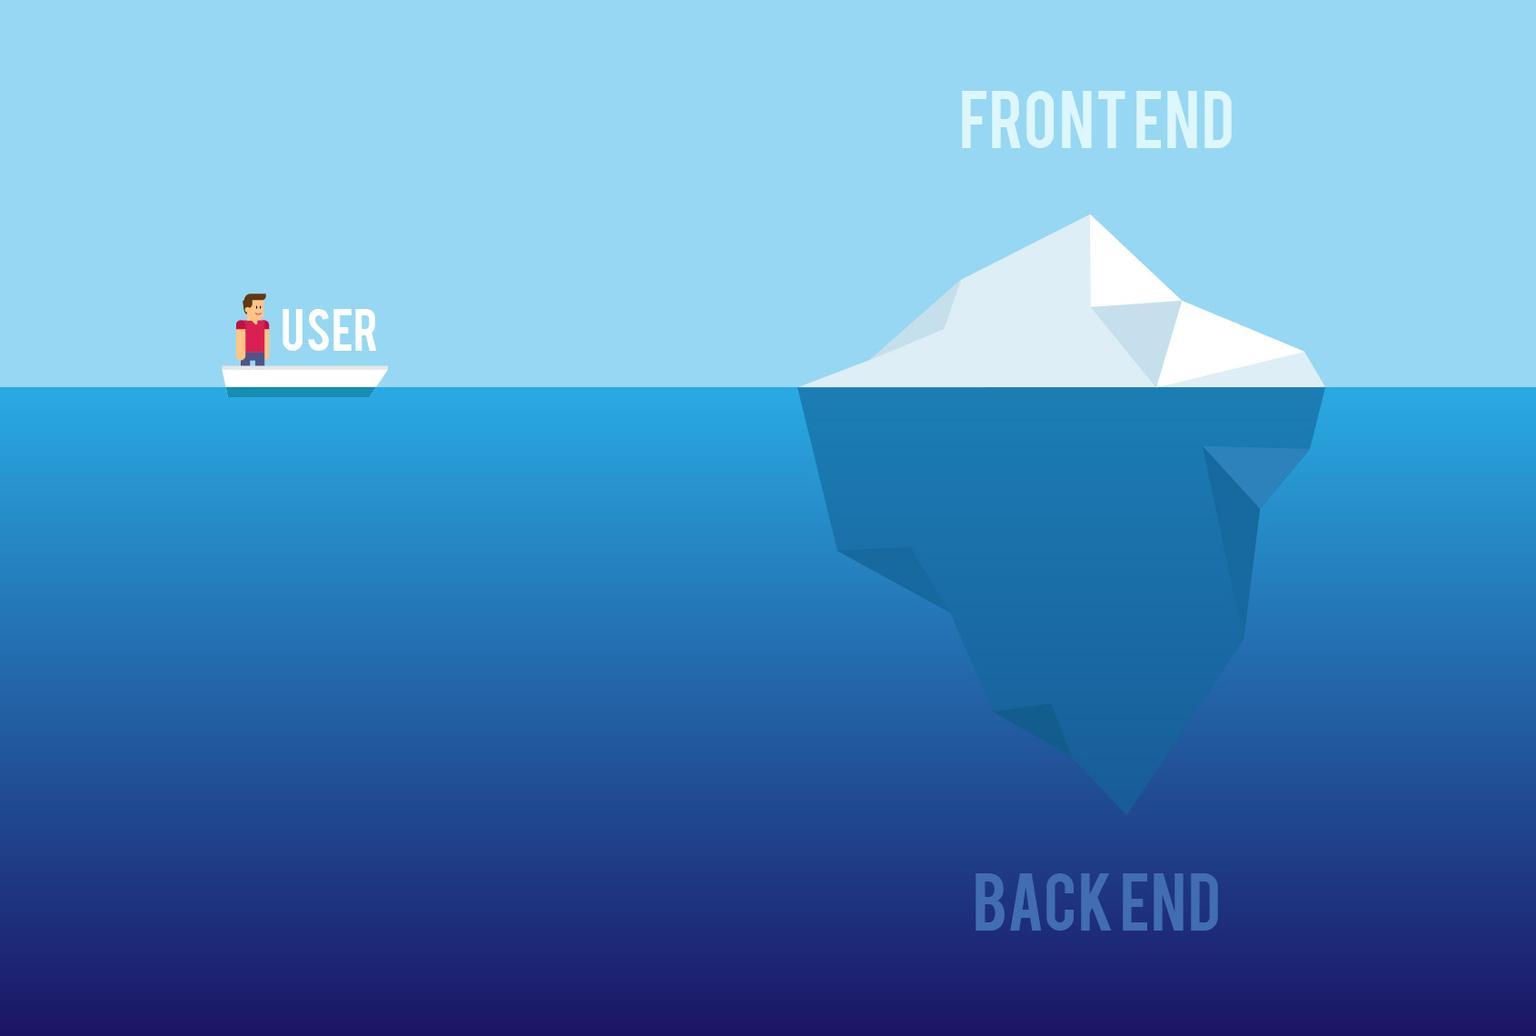
\includegraphics[scale=0.11]{img/front-back.jpg}
		\end{figure}
	\end{frame}

	\begin{frame}\frametitle{Aplicação Web}
		\begin{itemize}
			\item Os \textit{Frameworws} são esqueletos de uma aplicação e possuem conjuntos já definidos e diversas estruturas prontas.
			\item \textit{Representational State Transfer} (REST) é uma arquitetura baseado no protocolo \textit{HyperText Transfer Protocol} (HTTP) que serve para definir como é a comunicação entre sistemas de informação e a transferência de dados entre eles.
		\end{itemize}
	\end{frame}


	\begin{frame}\frametitle{Ferramentas}
		\begin{itemize}
			\item As linguagens de programação são utilizadas como meio de comunicação entre computadores e desenvolvedores.
			\item Um sistema de banco de dados é um sistema computadorizado de manutenção de registros cuja finalidade é armazenar informações e permitir que o usuário busque e atualize essas informações quando solicitado.
		\end{itemize}
	\end{frame}

	\begin{frame}\frametitle{Ferramentas}
		Application Programming Interface (API) é um conjunto estabelecido de mensagem que utilizam os métodos HTTP.
			\begin{figure}[ht]
				\centering
				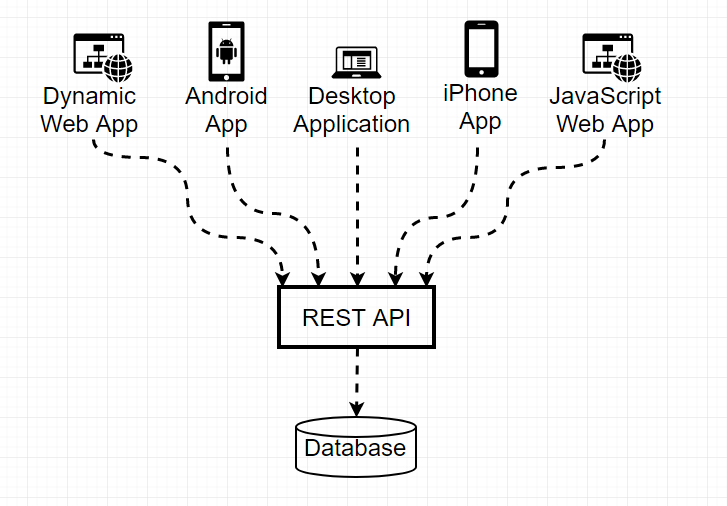
\includegraphics[scale=0.3]{img/rest_api.png}
			\end{figure}
	\end{frame}

	\begin{frame}\frametitle{Tecnologias}
		\begin{itemize}
			\item Java é uma linguagem de programação que pode ser utilizada para programar sistemas computacionais em alto nível.
			\item O Spring boot é um framework que acelera a programação de aplicações Java.
			\item O \textit{Hibernate} permite a comunicação entre a aplicação e o banco de dados através de \textit{Java Persistence API} (JPA). JPA permite à aplicação.
			\item O MySQL é um Sistema Gerenciador de Bancos de Dados (SGBD).
		\end{itemize}
	\end{frame}

	\begin{frame}\frametitle{Tecnologias}
		\begin{itemize}
			\item O \textit{Hypertext Markup Language} (HTML) é uma linguagem de marcação que serve para estruturar a apresentação e conteúdo.
			\item A estilização do HTML pode ser feita através de \textit{Cascading Style Sheets} (CSS).
			\item JavaScript é uma linguagem de programação. Uma de suas principais funcionalidades é fornecer interatividade nas aplicações originalmente estáticas.
			\item O \textit{Bootstrap} é um \textit{framework} que é utilizado para a padronização de interface da aplicação, ele é composto por componentes HTML, CSS, e JavaScript.
			\item O AngularJS é um \textit{framework} JavaScript que pode ser usado para o desenvolvimento de aplicações web e mobile.
		\end{itemize}
	\end{frame}

	\begin{frame}\frametitle{Homologação e Implantação}
		\begin{itemize}
		\item A homologação é a fase onde o cliente e os interessados pelo produto, verificaram que o software feito atende aos critérios de aceite previamente estabelecidos com o cliente.
		\item Após a aprovação do cliente o produto é entregue, e o cliente pode implantar o software em seu ambiente de produção.
		\end{itemize}
	\end{frame}

	\begin{frame}\frametitle{Homologação e Implantação}
		Para controlar as versões, o produto obedece a um modelo chamado versionamento semântico.
		\begin{itemize}
			\item X(Maior): quando ocorrem mudanças incompatíveis.
			\item Y(Menor): quando são adicionadas funcionalidades mantendo compatibilidade.
			\item Z(Correção): quando são corrigidas as falhas mantendo compatibilidade.
		\end{itemize}
	\end{frame}

	\begin{frame}\frametitle{Homologação e Implantação}
		Quando um software é lançado recebe a o número de versão 1.0.0. O maior (X) geralmente é usado para uma nova versão de software que recebera grandes modificações.
		Quando o software recebe melhorias o menor (Y) é adicionado 1.1.0 e quando recebe correções é adicionado o correção (Z) correção 1.1.1.
	\end{frame}

	\begin{frame}\frametitle{Processo de software}
		Processo de software é um conjunto de atividades e resultados associados que produzem um produto de software.
		\begin{itemize}
			\item Especificação de software
			\item Design e implementação do software
			\item Verificação e validação
			\item Manutenção do software
		\end{itemize}
	\end{frame}

	\section{Método}
	
		\begin{frame}\frametitle{Processo de software}
			
			O processo de desenvolvimento de software é algo complexo devido a variáveis que podem ter diferentes perspectivas de resultados.
		\end{frame}
	
		\begin{frame}\frametitle{Levantamento de requisitos}
			Através do levantamento de requisitos determinamos os problemas
			\begin{itemize}
				\item Problemas
				\item Soluções
			\end{itemize}
		\end{frame}
	
		\begin{frame}\frametitle{Implementação do sistema}
			A implementação da aplicação foi baseada em uma stack (pilha) de programas.
			\begin{figure}[ht]
				\centering
				\includegraphics[scale=0.3]{img/arquitetura.png}
			\end{figure}
		\end{frame}
	
		\begin{frame}\frametitle{Implantação do sistema}
			A implantação do sistema ainda não ocorreu.
		\end{frame}
	
	\section{Resultado}
		
		\begin{frame}\frametitle{Resultado}
			Vamos testar as funcionalidades.
			
			Os sistema está disponível no GitHub no endereço: <https://github.com/dragao1995/
			licitacaoweb> sob a Licença Apache 2.0.
		\end{frame}

	\section{Conclusão}
	
		\begin{frame}\frametitle{Conclusão}
			Foi desenvolvida uma aplicação web que tem o objetivo de melhorar a comunicação na fase interna de um processo de licitação.
		\end{frame}	
	
	\section{Obrigado}
		
\end{document}
